\documentclass[a4paper,11pt]{article}
\usepackage{graphicx}
\usepackage{booktabs}
\usepackage{setspace}
\usepackage{parskip}
\onehalfspacing
\begin{document}

\author{Hiromasa Okada}
\title{\vspace{-2cm}Report for Sheet 3\\
\small{Lab Course Machine Learning and Data Analysis}}
\maketitle

\section*{Implementation comments}
In this exercise I implemented Cross-validation function 

\begin{verbatim}
def cv(X, y, method, parameters, nfolds, nrepetitions, loss function)
\end{verbatim}
and Kernel Ridge Regression class 

\begin{verbatim}
class krr(kernel, kernelparameter, regularization)
\end{verbatim}

The cross validation function will find the best parameter combination for Kernel Ridge Regression during compute loss of the prediction.


\begin{verbatim}



\end{verbatim}


\section*{Assignment 3}

\begin{figure}[htbp]
  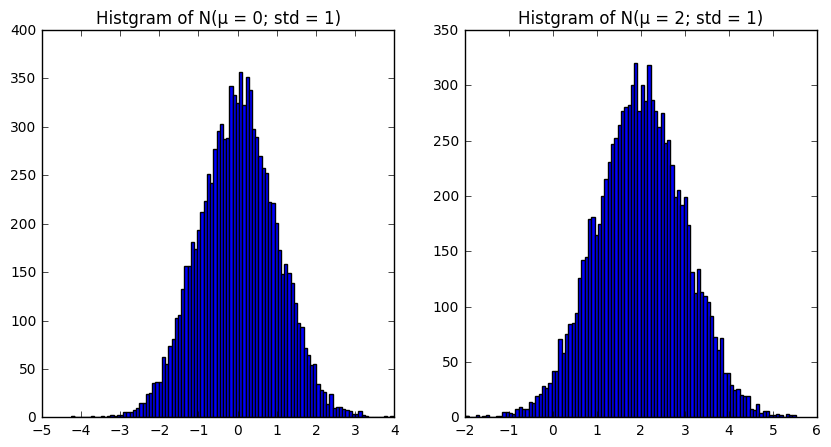
\includegraphics[scale=0.5]{hist12.png}
  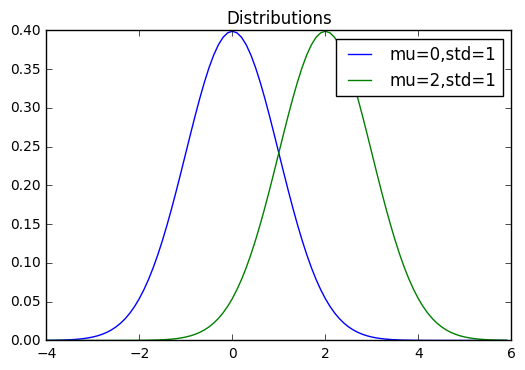
\includegraphics[scale=1.]{histmix.png}
  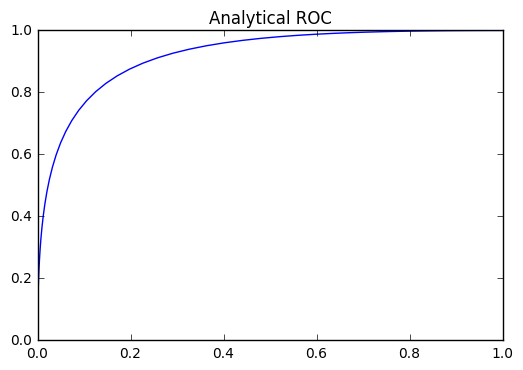
\includegraphics[scale=1.]{roc.png}
\end{figure}
\section*{Assignment 4}
\subsection*{Inv or Solve}


\begin{eqnarray*}
X=
\left(
\begin{array}{cccc}
2 & 4 & 6 \\
8 & 10 & 12  
\end{array}
\right)
, \:\:\:\:
\mu = 
\left(
\begin{array}{cccc}
4  \\
10  
\end{array}
\right) 
\end{eqnarray*}
\begin{eqnarray*}
C &=&
\left(
\begin{array}{cccc}
-2 & 0 & 2 \\
-2 & 0 & 2  
\end{array}
\right) 
\left(
\begin{array}{cccc}
-2 & -2\\
0 & 0 \\
2 & 2  
\end{array}
\right) 
= 
\left(
\begin{array}{cccc}
8 & 8\\
8 & 8 \\  
\end{array}
\right) \\
&\Rightarrow& \det(C) =0
\end{eqnarray*}





\end{document}

